\pgfplotsset{compat=1.17}
\usepgfplotslibrary{fillbetween}
\newcommand\samples{1}

\begin{figure}
    \centering
    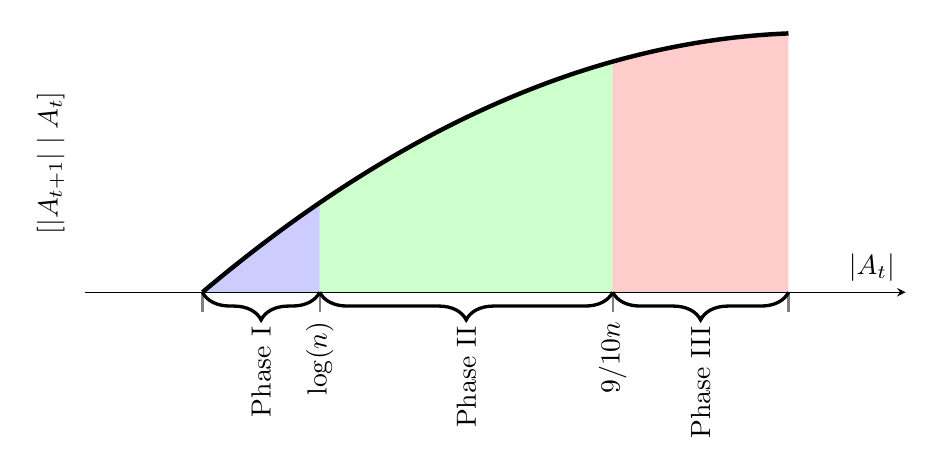
\begin{tikzpicture}[declare function={f(\x)=\x*(1 + (1-pow(0.3,2))*(1 - \x/100));}]
    \begin{axis}[width=12cm,
                 height=5cm,
                 axis x line=middle,
                 axis y line=left,
                 enlarge x limits=0.2,
                 enlarge y limits=0.02,
                 y axis line style ={opacity=0},
                 ytick=\empty,
                 xtick={0,20, 70,100},
                 xticklabels={,$\log(n)$, $9/10n$, },
                 x tick style={thick},
                 xtick align=outside,
                 tickwidth=0.25cm,
                 x tick label style={rotate=90,anchor=east},
                 xlabel={$|A_t|$},
                 ylabel={$\E\left[|A_{t+1}| \mid A_t\right]$}, 
                 very thick]
    
    \addplot[name path=graph, ultra thick, domain=0:100, smooth, samples=100*\samples]{f(x)}; 
    \addplot[name path=axis, very thick, domain=0:100, smooth, draw opacity =0, samples=100*\samples]{0}; 
    \addplot [thick, color=blue, fill=blue, fill opacity=0.2]
    fill between[of=graph and axis, soft clip={domain=0:20}];
    \addplot [thick, color=green, fill=green, fill opacity=0.2]
    fill between[of=graph and axis, soft clip={domain=20:70}];
    \addplot [thick, color=red, fill=red, fill opacity=0.2]
    fill between[of=graph and axis, soft clip={domain=70:100}];

    \path (0,0) coordinate (O) (20,0) coordinate (A) (70,0) coordinate (B) (100,0) coordinate (C);

    
    \end{axis}
    \draw [very thick, black, decorate,decoration={brace,amplitude=10pt,mirror},xshift=0.4pt,yshift=-0.4pt] (O) -- (A) node[black,anchor=east,midway,yshift=-0.3cm,rotate=90] {Phase I};
    \draw [very thick, black, decorate,decoration={brace,amplitude=10pt,mirror},xshift=0.4pt,yshift=-0.4pt] (A) -- (B) node[black,anchor=east,midway,yshift=-0.3cm,rotate=90] {Phase II};
    \draw [very thick, black, decorate,decoration={brace,amplitude=10pt,mirror},xshift=0.4pt,yshift=-0.4pt] (B) -- (C) node[black,anchor=east,midway,yshift=-0.3cm,rotate=90] {Phase III};

    \end{tikzpicture}    
\caption{Growth of BIPS, as given by the lower bound in Lemma~\ref{lemma:bips-growth}. In phase I, the active set is sublogarithmic. In phase II the active set is at least logarithmic and at most $9/10n$. In phase III, and the active set is at least $9/10n$ and reaches size $n$ at the end. Each phase takes $O(\log(n))$ rounds.}
    \label{fig:growth-bips}
\end{figure}
